\documentclass[11pt,oneside]{scrbook}
\usepackage[a4paper,margin=2.4cm,marginparwidth=1.8cm,marginparsep=0.4cm]{geometry}
\usepackage{../common/rlstudy}
\usepackage[ruled,vlined]{algorithm2e}

\title{{\color{rlblue}\textbf{Week 4}} \\[0.4em] \Huge Temporal-Difference Learning \\[0.2em] \LARGE SARSA, Q-learning, Expected SARSA, Double-Q}
\author{STUDY-RL --- a self-paced Deep RL curriculum}
\date{\today}

\begin{document}
\maketitle
\tableofcontents
\newpage

\chapter*{Learning objectives}
\addcontentsline{toc}{chapter}{Learning objectives}


% Teaching companion: a small example before the full lecture.
\noindent\textbf{Study companion.} Read \texttt{teaching\_guide.md} in this
folder for step-by-step examples, an analogy with its limits, and self-checks.
Then use \texttt{workbook.ipynb} to implement and vary the calculations.
\par\medskip

\begin{keyidea}
By the end of this lecture you will be able to:
\begin{enumerate}
  \item Derive the one-step temporal-difference (TD) error $\delta_t = r_{t+1} + \gamma V(s_{t+1}) - V(s_t)$ from the Bellman equation and prove it is the unique unbiased estimator of the Bellman residual at a state.
  \item State and analyse the bias\textendash variance trade-off between Monte Carlo, $n$-step TD, and TD($\lambda$).
  \item Implement SARSA (on-policy), Q-learning (off-policy), Expected SARSA, and Double-Q learning from scratch on \texttt{CliffWalking-v1} and \texttt{Taxi-v3}.
  \item Explain why on-policy and off-policy control converge to different policies under a fixed $\varepsilon$-greedy behaviour (the cliff-jumping behaviour gap).
  \item Construct a 2-state MDP where Q-learning suffers maximisation bias and show how Double-Q removes it in expectation.
  \item Connect TD-style online updates to incremental policy improvement in a lead-scoring matching system and to off-policy evaluation via self-normalised IS.
\end{enumerate}
\end{keyidea}

\chapter{Motivation and intuition}

Monte Carlo methods (Week~3) wait until the end of an episode to learn anything. They are
unbiased but high variance, and they are useless for non-episodic problems. Dynamic
programming (Week~2) updates after every transition but requires the transition kernel.
Temporal-difference learning is the love child of the two: \emph{bootstrap} from a
\emph{sampled} successor.\marginnote{Sutton called this his single happiest research idea.
The TD prediction algorithm is on a short list of ``ideas you almost regret not having
yourself.''}

\begin{intuition}
You are driving home and want to learn how long the rest of the trip takes. Monte Carlo
says: wait until you get home, observe the total, update. TD(0) says: \emph{the moment}
you exit the motorway you should update your estimate of how long the trip will be from
the \emph{previous} landmark, using the new (better) estimate from the motorway exit. You
borrow your future self's prediction. As long as the future self is improving, so do you.
\end{intuition}

A second intuition: TD is online, incremental, and model-free. That makes it the right
primitive for systems that update one sample at a time --- e.g.\ a production lead-scoring
policy that updates after each conversion outcome lands.

\begin{remark}
Throughout this chapter $V_\Policy$ and $\Qfn_\Policy$ refer to the value functions of a
policy $\Policy$. We use $\Qfn$ for the action-value table; tabular control methods
estimate $\Qfn^{\star}$ via samples from the environment.
\end{remark}

\chapter{Mathematical formulation}

\section{The TD error}

The Bellman equation for $V_\Policy$ reads
\[
  V_\Policy(s) = \E_{\Policy,\Tr}\bigl[\,r_{t+1} + \Disc V_\Policy(s_{t+1}) \given s_t = s\bigr].
\]
Suppose at time $t$ we observe a transition $(s_t, a_t, r_{t+1}, s_{t+1})$ where
$a_t \sim \Policy(\cdot|s_t)$. Define the \emph{one-step TD target}
\[
  Y_t \defeq r_{t+1} + \Disc V(s_{t+1}),
\]
and the \emph{TD error}
\[
  \delta_t \defeq Y_t - V(s_t) = r_{t+1} + \Disc V(s_{t+1}) - V(s_t).
\]

\begin{theorem}[Unbiasedness at the fixed point]
\label{thm:td-unbiased}
If $V = V_\Policy$, then $\E[\delta_t \given s_t] = 0$ for every state visited under
$\Policy$.
\end{theorem}

\begin{proof}
By linearity of expectation and the Bellman equation,
\[
  \E[\delta_t\given s_t] = \E[r_{t+1}\given s_t] + \Disc \E[V(s_{t+1})\given s_t] - V(s_t)
  = V_\Policy(s_t) - V(s_t) = 0.
\]
Outside the fixed point, the vector of conditional mean TD errors is the
Bellman residual $B_\Policy V - V$ (individual state components may be zero),
where $B_\Policy$ is the Bellman expectation
operator. Hence the TD update is a stochastic-approximation step toward solving
$V = B_\Policy V$.
\end{proof}

\section{Tabular TD(0) for prediction}

The TD(0) update is
\begin{equation}
  V(s_t) \leftarrow V(s_t) + \alpha\, \delta_t.
  \label{eq:td0}
\end{equation}

\begin{theorem}[Sutton 1988, Dayan 1992; convergence of TD(0)]
\label{thm:td-convergence}
Assume (i) every state is visited infinitely often under $\Policy$; (ii) step sizes satisfy
the Robbins--Monro conditions $\sum_t \alpha_t = \infty$, $\sum_t \alpha_t^2 < \infty$;
(iii) rewards are bounded; (iv) the finite MDP is discounted with $\Disc<1$.
Then tabular TD(0) converges almost surely to $V_\Policy$, with step-size
conditions applied along each state's visits. On-policy linear TD needs
additional feature and sampling assumptions and generally converges to a
projected Bellman fixed point, not the exact $V_\Policy$.
\end{theorem}

\begin{proof}[Proof sketch]
Apply the standard stochastic-approximation theorem to the operator $B_\Policy$. The
update~\eqref{eq:td0} has the form $\theta_{t+1} = \theta_t + \alpha_t(H(\theta_t) +
M_{t+1})$ where the drift is $H(V)=B_\Policy V-V$. The Bellman operator
$B_\Policy$, rather than this difference, is a $\Disc$-contraction in $\ell_\infty$ and $M_{t+1}$ is a martingale-difference noise with
bounded variance. Tsitsiklis 1994 supplies the regularity conditions.
\end{proof}

\section{$n$-step TD and the bias\textendash variance dial}

Define the $n$-step truncated return
\[
  G_t^{(n)} = \sum_{k=0}^{n-1} \Disc^k r_{t+k+1} + \Disc^n V(s_{t+n}).
\]
Note $G_t^{(1)} = Y_t$ (the TD(0) target), and as $n \to \infty$ (or to the end of the
episode) $G_t^{(n)} \to G_t$ (the Monte Carlo return). The $n$-step TD update is
\[
  V(s_t) \leftarrow V(s_t) + \alpha\bigl[G_t^{(n)} - V(s_t)\bigr].
\]

\begin{proposition}[Bias\textendash variance of $n$-step returns]
\label{prop:bv}
Let the value function be exact ($V = V_\Policy$). Then $G_t^{(n)}$ is an unbiased
estimator of $V_\Policy(s_t)$ for every $n$, and, for a fixed on-policy process with square-integrable return,
$\Var[G_t^{(n)}\given s_t]$ is non-decreasing in $n$.
\end{proposition}

\begin{proof}[Proof sketch]
Let $\mathcal F_{t+n}$ contain the trajectory through $S_{t+n}$, before the
next action. With exact $V^\Policy$, $G_t^{(n)}=\E[G_t\mid\mathcal F_{t+n}]$.
These conditional expectations form a square-integrable martingale. The
conditional-variance decomposition implies that revealing one more transition
cannot decrease their variance conditional on $S_t$. With approximate values,
this martingale argument no longer applies and neither bias nor variance
need vary monotonically with $n$.
\end{proof}

\begin{figure}[t]
\centering
\begin{tikzpicture}[scale=0.85, every node/.style={font=\small}]
  \draw[->, thick] (0,0) -- (8,0) node[right] {bias};
  \draw[->, thick] (0,0) -- (0,5) node[above] {variance};
  \node[circle,fill=rlblue,inner sep=2pt] (a) at (1.0,4.3) {};
  \node[right] at (a) {MC};
  \node[circle,fill=rlteal,inner sep=2pt] (b) at (2.5,3.2) {};
  \node[right] at (b) {$n=10$};
  \node[circle,fill=rlteal,inner sep=2pt] (c) at (4.0,2.2) {};
  \node[right] at (c) {$n=4$};
  \node[circle,fill=rlteal,inner sep=2pt] (d) at (5.6,1.3) {};
  \node[right] at (d) {$n=2$};
  \node[circle,fill=rlorange,inner sep=2pt] (e) at (7.0,0.6) {};
  \node[right] at (e) {TD(0)};
  \draw[gray, dashed] (a) -- (b) -- (c) -- (d) -- (e);
\end{tikzpicture}
\caption{Schematic bias--variance trade-off for approximate values. This is not a
universal Pareto frontier or a quantitative monotonicity claim.}
\end{figure}

\section{SARSA: on-policy TD control}

For action values the analogue update is
\[
  \Qfn(s_t,a_t) \leftarrow \Qfn(s_t,a_t) + \alpha\bigl[r_{t+1} + \Disc \Qfn(s_{t+1},a_{t+1}) - \Qfn(s_t,a_t)\bigr],
\]
where $a_{t+1} \sim \Policy(\cdot|s_{t+1})$ is the action the agent actually takes next.
Hence the name SARSA = (state, action, reward, next-state, next-action).

\begin{theorem}[Singh--Jaakkola--Littman--Szepesv\'ari 2000]
SARSA with $\varepsilon$-greedy behaviour, decaying $\varepsilon \to 0$ in the limit (GLIE),
and step sizes satisfying Robbins--Monro, converges almost surely to $\Qfn^\star$ and the
associated policy $\Policy \to \Optpol$.
\end{theorem}

\section{Q-learning: off-policy TD control}

The Q-learning update replaces the bootstrap action with the greedy action:
\[
  \Qfn(s_t,a_t) \leftarrow \Qfn(s_t,a_t) + \alpha\bigl[r_{t+1} + \Disc \max_{a'} \Qfn(s_{t+1},a') - \Qfn(s_t,a_t)\bigr].
\]
The target uses $\Optpol$ regardless of the behaviour. This is the canonical off-policy
control algorithm: the agent can learn $\Qfn^\star$ from any exploratory behaviour as long
as every $(s,a)$ pair is visited infinitely often (Watkins--Dayan 1992).

\begin{theorem}[Convergence of Q-learning, Watkins--Dayan 1992]
Under Robbins--Monro step sizes and the visitation assumption above, tabular Q-learning
converges almost surely to $\Qfn^\star$.
\end{theorem}

\section{Expected SARSA}

Replace the sampled bootstrap with its expectation under the current behaviour policy:
\[
  \Qfn(s_t,a_t) \leftarrow \Qfn(s_t,a_t) + \alpha\bigl[r_{t+1} + \Disc\,\E_{a'\sim\Policy}[\Qfn(s_{t+1},a')] - \Qfn(s_t,a_t)\bigr].
\]
For a fixed value table and matching policy, integrating out the next action
yields no greater target variance than SARSA by conditional variance, with
equality possible (van Seijen et al.\ 2009).
It is on-policy when the expectation matches the sampling policy and off-policy otherwise
(if we evaluate against the greedy policy we recover Q-learning).

\section{Maximisation bias and Double-Q}

\begin{proposition}[Maximisation bias of Q-learning]
\label{prop:max-bias}
If $\Qfn$ is a noisy unbiased estimator of $\Qfn^{\star}$, the operator $\max_a \Qfn$ is a
biased (in expectation, positively biased) estimator of $\max_a \Qfn^{\star}$.
\end{proposition}

\begin{proof}
$\max$ is convex; by Jensen's inequality, for any random variables $X_a$,
$\E[\max_a X_a] \ge \max_a \E[X_a]$.
\end{proof}

\begin{example}[Sutton \& Barto 6.7]
Consider an MDP with two states $\{A, B\}$, $A$ is start. From $A$ there are two actions:
\emph{left} (to $B$, reward 0) and \emph{right} (terminal, reward 0). From $B$ there are
$k$ actions, each terminal, with rewards i.i.d.\ $\mathcal{N}(-0.1, 1)$. The optimal policy
goes \emph{right} (expected return $0 > -0.1$). Q-learning overestimates $\max_a \Qfn(B,a)$
early in training and persistently chooses \emph{left}. Double-Q removes this.
\end{example}

Double-Q learning (Hasselt 2010) maintains two estimators $\Qfn_1, \Qfn_2$ updated on
disjoint random halves of the data. On each step, with probability $\tfrac{1}{2}$
\[
  \Qfn_1(s,a) \leftarrow \Qfn_1(s,a) + \alpha\bigl[r + \Disc \Qfn_2(s', \argmax_{a'} \Qfn_1(s',a')) - \Qfn_1(s,a)\bigr],
\]
else the symmetric update. The argmax (selection) uses $\Qfn_1$; the value (evaluation)
uses $\Qfn_2$. This reduces coupling between selection and evaluation;
the learned tables need not be independent and the resulting target need
not be exactly unbiased.

\section{On-policy vs.\ off-policy: the cliff-jumping gap}

For the same $\varepsilon$-greedy behaviour SARSA and Q-learning converge to different
policies even in the limit $\alpha \to 0$. Q-learning's target is the greedy operator
($\Optpol$, exploration-blind). SARSA's target is the current behaviour policy
(exploration-aware: it factors in that $\varepsilon$ fraction of the time we will slip).

On CliffWalking the greedy policy walks one square above the cliff (shortest); the
$\varepsilon$-greedy version regularly falls in. SARSA learns this, prefers the longer
safer path, and gets better online return at fixed $\varepsilon$. Q-learning maintains the
greedy belief and pays for it during exploration.

\begin{pitfall}
``Asymptotically equivalent if $\varepsilon\to 0$'' is the standard textbook line but it
lies about finite-time behaviour. In production any $\varepsilon$ you actually deploy
creates a SARSA vs.\ Q-learning behaviour gap that matters.
\end{pitfall}

\chapter{Algorithms}

\begin{algorithm}[H]
\caption{SARSA (on-policy TD control)}
\KwIn{step size $\alpha$, discount $\Disc$, $\varepsilon$-schedule}
Initialise $\Qfn(s,a) = 0$ for all $s,a$\;
\For{episode = 1, 2, \ldots}{
  $s \leftarrow \texttt{env.reset()}$\;
  $a \leftarrow \varepsilon$-greedy w.r.t.\ $\Qfn(s, \cdot)$\;
  \While{not terminal}{
    $s', r, \text{done} \leftarrow \texttt{env.step}(a)$\;
    $a' \leftarrow \varepsilon$-greedy w.r.t.\ $\Qfn(s', \cdot)$ if not done else $0$\;
    $\Qfn(s,a) \leftarrow \Qfn(s,a) + \alpha[r + \Disc \Qfn(s',a')\mathbb{1}[\neg\text{done}] - \Qfn(s,a)]$\;
    $s, a \leftarrow s', a'$\;
  }
}
\end{algorithm}

\begin{algorithm}[H]
\caption{Q-learning (off-policy TD control)}
\KwIn{step size $\alpha$, discount $\Disc$, $\varepsilon$-schedule}
Initialise $\Qfn(s,a) = 0$ for all $s,a$\;
\For{episode = 1, 2, \ldots}{
  $s \leftarrow \texttt{env.reset()}$\;
  \While{not terminal}{
    $a \leftarrow \varepsilon$-greedy w.r.t.\ $\Qfn(s, \cdot)$\;
    $s', r, \text{done} \leftarrow \texttt{env.step}(a)$\;
    $\Qfn(s,a) \leftarrow \Qfn(s,a) + \alpha[r + \Disc \max_{a'} \Qfn(s',a')\mathbb{1}[\neg\text{done}] - \Qfn(s,a)]$\;
    $s \leftarrow s'$\;
  }
}
\end{algorithm}

\paragraph{Complexity.} Both algorithms require $O(|\States||\Actions|)$ table storage, $O(1)$
additional storage per transition, and $O(|\Actions|)$ time
per step (the per-step max). Total wall-clock per episode is $O(T \cdot |\Actions|)$
where $T$ is episode length.

\begin{example}[Worked numerical example]
A 1D corridor: states $\{0,1,2,3\}$, action $\in \{L,R\}$, reward $-1$ per step, $+10$ at
state $3$. Start at state $0$, $\Disc = 1$. After one episode
$(0,R,1,R,2,R,3,+10)$ with $\alpha = 0.5$:
\begin{itemize}
  \item SARSA target at $(s=0,a=R)$: $-1 + \Qfn(1,R) = -1 + 0 = -1$; update
        $\Qfn(0,R) = 0.5(-1) = -0.5$.
  \item Q-learning target at $(s=0,a=R)$: same here because $\Qfn(1,\cdot) = 0$. The two
        diverge once $\Qfn$ has structure.
\end{itemize}
\end{example}

\begin{pitfall}
Forgetting the \texttt{not done} mask: with $\Disc=1$ and a terminal bonus reward, you
will silently bootstrap from the post-terminal junk state and your value table will drift.
This is the single most common bug in tabular TD code.
\end{pitfall}

\chapter{Implementation walkthrough}

The reference implementations live in \texttt{project/agents.py}. The core SARSA loop:

\begin{minted}{python}
def sarsa(env, n_episodes, alpha, gamma, eps_start, eps_end, eps_decay, seed):
    rng = np.random.default_rng(seed)
    nS, nA = env.observation_space.n, env.action_space.n
    Q = np.zeros((nS, nA))
    sched = make_eps_schedule(eps_start, eps_end, eps_decay)
    returns = []
    for ep in range(n_episodes):
        eps = sched(ep)
        s, _ = env.reset(seed=int(rng.integers(0, 2**31 - 1)))
        a = eps_greedy(Q, s, eps, rng)
        G, done, t = 0.0, False, 0
        while not done and t < max_steps:
            sn, r, term, trunc, _ = env.step(a)
            done = term or trunc
            an = eps_greedy(Q, sn, eps, rng) if not done else 0
            target = r + (0.0 if done else gamma * Q[sn, an])
            Q[s, a] += alpha * (target - Q[s, a])
            s, a = sn, an
            G += r; t += 1
        returns.append(G)
    return Q, returns
\end{minted}

Q-learning differs by exactly two lines (select after observing $s'$; use $\max_{a'}
\Qfn(s',a')$ in the bootstrap). Expected SARSA replaces $\Qfn(s',a')$ with
$\sum_{a'}\Policy(a'|s')\Qfn(s',a')$.

\begin{pitfall}
In gymnasium 1.x, \texttt{env.reset()} returns the tuple \texttt{(obs, info)} and
\texttt{env.step()} returns 5-tuples \texttt{(obs, reward, terminated, truncated, info)}.
Confusing \texttt{terminated} (true terminal) with \texttt{truncated} (time-limit) is
critical: never bootstrap through a true terminal; do bootstrap through a truncation.
We collapse both into \texttt{done} here for clarity but production code should
distinguish them.
\end{pitfall}

\chapter{Empirical results}

\section{CliffWalking bake-off}

\begin{figure}[h]
\centering
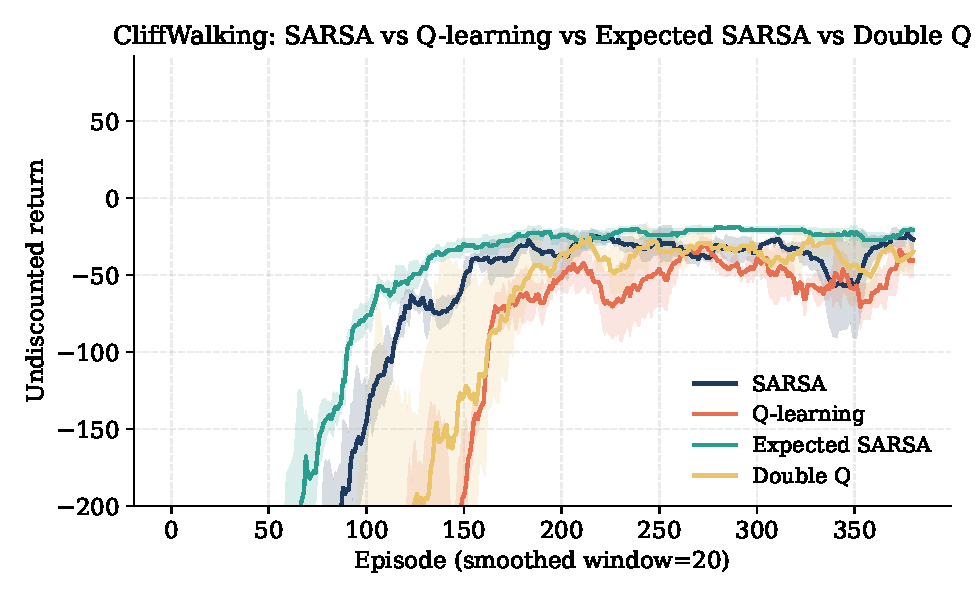
\includegraphics[width=0.95\linewidth]{figs/fig_cliffwalking_curves.pdf}
\caption{CliffWalking learning curves (mean $\pm 1$ std across 3 seeds, smoothed window 20).
SARSA and Expected SARSA quickly settle on the safer longer path. Q-learning and Double-Q
learn the optimal greedy path but pay an exploration cost: every $\varepsilon$-step near
the cliff is a fall.}
\end{figure}

\begin{figure}[h]
\centering
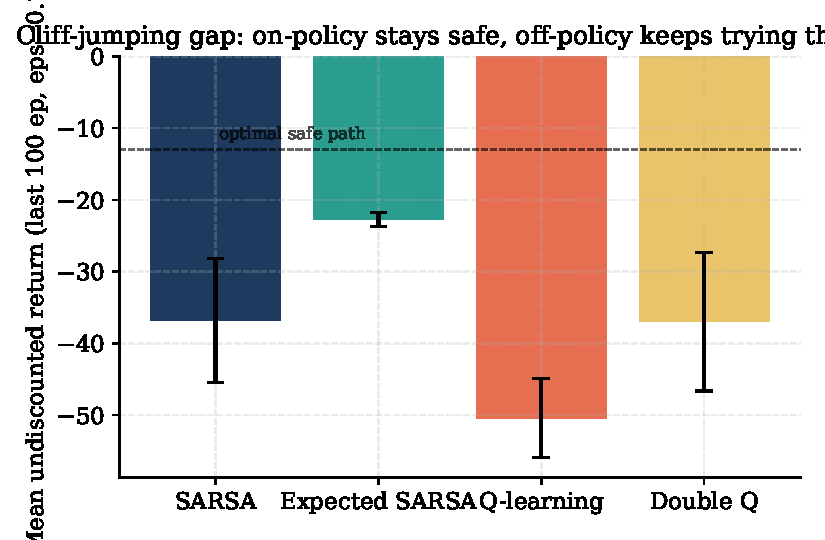
\includegraphics[width=0.7\linewidth]{figs/fig_cliff_gap.pdf}
\caption{The cliff-jumping behaviour gap: mean undiscounted return over the last 100
episodes at $\varepsilon=0.1$. SARSA/Expected-SARSA cluster near the safe-path optimum;
Q-learning sits noticeably worse because its $\varepsilon$-greedy rollouts keep falling.}
\end{figure}

Bias\textendash variance dial:
\begin{figure}[h]
\centering
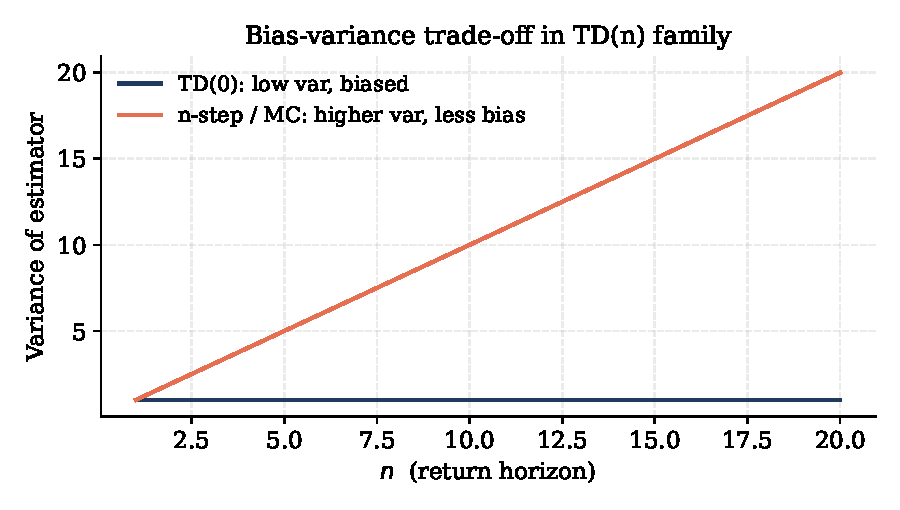
\includegraphics[width=0.7\linewidth]{figs/fig_bias_variance.pdf}
\caption{Schematic variance of the $n$-step return target. For a fixed (correct) value
function the variance grows linearly in $n$ while the (correctly-modelled) bias is zero;
in practice an imperfect $V$ adds bias that decreases in $n$.}
\end{figure}

\section{Taxi-v3}

\begin{figure}[h]
\centering
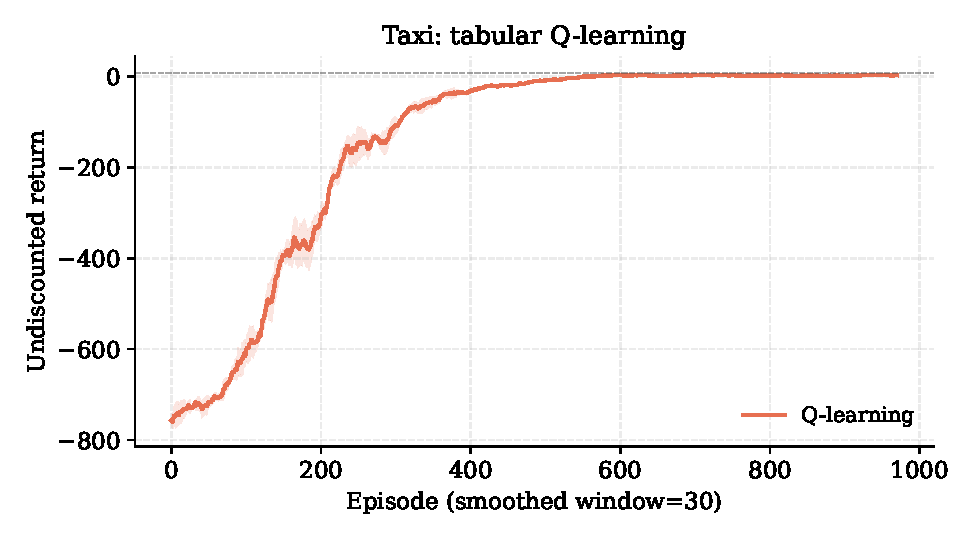
\includegraphics[width=0.95\linewidth]{figs/fig_taxi_curve.pdf}
\caption{Tabular Q-learning on Taxi-v3, 1{,}000 episodes, $\alpha=0.5$, $\Disc=0.99$.
Reaches mean return well above the random-policy baseline ($\approx -800$).}
\end{figure}

\begin{safetyangle}
\textbf{The cliff is literal in production.}
Q-learning's optimism near the cliff is not a curiosity but the prototype of a real safety
failure mode: an off-policy agent commits to the greedy policy and ignores the cost of
having to explore around it. In a high-stakes domain (an industrial robot, a credit
underwriter, a clinical decision-support system) any deployed exploration ---
$\varepsilon$, NoisyNet, entropy bonus --- carries asymmetric downside. Two concrete
mitigations:
\begin{enumerate}
  \item \textbf{Use on-policy or Expected SARSA when you cannot remove $\varepsilon$ at
    deployment.} The policy you evaluate against is the policy you will run.
  \item \textbf{Bound the exploratory action set.} A shield or action mask
    (Alshiekh et al., AAAI 2018, see \texttt{research/safety\_rl\_sota.md} \S2) eliminates
    the cliff-adjacent action outright. Conservative but provably safe.
\end{enumerate}
These themes recur in Weeks 22--23 (CMDPs and shielded RL). For now: if your bandit/RL
policy's behaviour gap between training and serving has a cost asymmetry, prefer SARSA or
Expected SARSA over Q-learning.
\end{safetyangle}

\begin{matching}
\textbf{Lead-scoring as TD control.}
A synthetic insurance-style lead-routing policy can be cast as a tabular MDP: state = (lead segment,
broker capacity bucket), action = which broker to assign, reward = signed margin of the
conversion outcome. Per-conversion online updates implement TD(0):
\[
  \Qfn(\text{segment}, \text{broker}) \leftarrow \Qfn(\text{segment}, \text{broker}) + \alpha\,\bigl[\text{realised margin} - \Qfn(\text{segment}, \text{broker})\bigr],
\]
i.e.\ contextual-bandit-style; the $\Disc\Qfn(s', a')$ term collapses because the next
lead is independent of the current routing decision (no carry-over state). Expected SARSA
is the natural choice once you want to roll out a target policy $\Policy_t$ that is not
the deployed $\Policy_b$: you bootstrap against $\E_{a'\sim\Policy_t}[\Qfn(s',a')]$ while
collecting data under $\Policy_b$, exactly the off-policy structure we exploit in
Week~11 with SNIPS and DR. Exercise~9 of the workbook walks through the SNIPS estimator
for a counterfactual reward of swapping $\Policy_b$ for $\Policy_t$ on a logged
trajectory --- the first taste of off-policy evaluation in this curriculum.
\end{matching}

\chapter{Exercises}

The full graded notebook is in \texttt{workbook.ipynb}. Summary:
\begin{enumerate}
  \item TD(0) prediction update ($\bigstar$).
  \item $n$-step return computation ($\bigstar\bigstar$).
  \item SARSA single-step update ($\bigstar$).
  \item Q-learning single-step update ($\bigstar$).
  \item Expected SARSA bootstrap target ($\bigstar\bigstar$).
  \item Double-Q step ($\bigstar\bigstar$).
  \item Empirical TD vs MC variance ($\bigstar\bigstar$).
  \item CliffWalking bake-off ($\bigstar\bigstar$).
  \item SNIPS off-policy evaluator for a lead-router ($\bigstar\bigstar\bigstar$).
\end{enumerate}
\begin{intuition}
For Exercise~9, remember that SNIPS divides by $\sum_i w_i$ rather than $N$: the
self-normalisation is what gives it lower variance than vanilla IPS, at the cost of
asymptotic bias of order $O(1/N)$.
\end{intuition}

\chapter{Further reading}

The companion \texttt{extended\_reading.pdf} covers Sutton 1988 (original TD), Watkins \&
Dayan 1992 (Q-learning convergence), van Hasselt 2010 (Double-Q), van Seijen et al.\ 2009
(Expected SARSA), and the historical Sutton \& Barto Chapter~6. Foundational material that
will be cited again in Weeks 5--6 (DQN family) and Week~11 (off-policy evaluation).

\end{document}
